\documentclass[review]{elsarticle}

\usepackage{natbib}
\usepackage{graphicx, subfigure}
\usepackage{dcolumn}% Align table columns on decimal point
\usepackage{bm}% bold math

\usepackage{lineno,hyperref, url}
\usepackage{indentfirst}
\usepackage{array, threeparttable}
\usepackage{multirow}
\usepackage{mathrsfs}
\usepackage{color}
\usepackage{amsmath, amssymb}
\modulolinenumbers[5]
\journal{Journal of \LaTeX\ Templates}

%%%%%%%%%%%%%%%%%%%%%%%
%% Elsevier bibliography styles
%%%%%%%%%%%%%%%%%%%%%%%
%% To change the style, put a % in front of the second line of the current style and
%% remove the % from the second line of the style you would like to use.
%%%%%%%%%%%%%%%%%%%%%%%

%% Numbered
%\bibliographystyle{model1-num-names}

%% Numbered without titles
%\bibliographystyle{model1a-num-names}

%% Harvard
%\bibliographystyle{model2-names.bst}\biboptions{authoryear}

%% Vancouver numbered
%\usepackage{numcompress}\bibliographystyle{model3-num-names}

%% Vancouver name/year
%\usepackage{numcompress}\bibliographystyle{model4-names}\biboptions{authoryear}

%% APA style
%\bibliographystyle{model5-names}\biboptions{authoryear}

%% AMA style
%\usepackage{numcompress}\bibliographystyle{model6-num-names}

%% `Elsevier LaTeX' style
\bibliographystyle{elsarticle-num}
%%%%%%%%%%%%%%%%%%%%%%%

\begin{document}

\begin{frontmatter}
	
\title{High order compact least-squares reconstruction}
\author{Ji Li}
\ead{leejearl@mail.nwpu.edu.cn}


\address{National Key Laboratory of Science and Technology on Aerodynamic Design and Research, Northwestern Polytechnical 
University, Xi'an, Shaanxi 710072, China}

\begin{abstract}
	Notes.
\end{abstract}
\end{frontmatter}

\section{Reconstruction polynomial}
The reconstruction polynomial based on the zero-mean basis can be expressed as 
\begin{equation}\label{eq:RCP}
	u^i(x,y)=\overline{u}^i+\sum_{l=1}^{DOF(k)}u^i_l\phi_{l,i}(x, y),
\end{equation}
where 
\begin{equation*}
	\begin{gathered}
		\overline{u}^i=\frac{1}{\|\Omega_i\|}\int_{\Omega_i}u(\bm{x})d\Omega,
		\quad \phi_{l,i}(x,y)=\Delta x^m_i\Delta y^n_i-\overline{\Delta x^m_i\Delta y^n_i},\\
		\Delta x_i=\frac{x-x_i}{h_i},\quad \Delta y_i=\frac{y-y_i}{h_i}, \quad 
		\overline{\Delta x^m_i\Delta y^n_i}=\frac{1}{\|\Omega_i\|}\int_{\Omega_i}\Delta x^m_i\Delta y^n_id\Omega.
	\end{gathered}
\end{equation*}
$h_i$ is the length scale for the non-dimensionalization ofthe basis functions to avoid growth of the condition number of the reconstruction matrix with grid refinement. For triangular grids, the length scale is defined as
\begin{equation}\label{eq:h}
	h_i=max(Rad_i, \sqrt{\|\Omega_i\|}),
\end{equation}
where $Rad_i$ is the radius of the circumcircle of the control volume $\Omega_i$. The freedom of $k$ order polynomial reads
\begin{equation}\label{dof_k}
	DOF(k)=\left(k+1\right)\left(k+2\right)/2-1.
\end{equation} 
According to Eq.~\eqref{eq:RCP}, a quadratic reconstruction $(k=2)$ polynomial can be rewritten as
\begin{equation}\label{eq:quadRCP}
	\begin{gathered}
		u^i(x,y)=\overline{u}^i+\sum_{l=1}^{5}u^i_l\phi_{l,i}(x, y)=\overline{u}^i+u^i_1\Delta x+u^i_2\Delta y\\
		+\frac{1}{2}u^i_3\left(\Delta x^2 - \overline{\Delta x^2_i}\right)
		+u^i_4\left(\Delta x\Delta y - \overline{\Delta x_i\Delta y_i}\right)
		+\frac{1}{2}u^i_5\left(\Delta y^2 - \overline{\Delta y^2_i}\right).
	\end{gathered}
\end{equation}
Because of the use of zero-mean basis, the following condition,
\begin{equation}\label{eq:cellAVGCond}
	\overline{u}^i=\frac{1}{\|\Omega_i\|}\int_{\Omega_i}u(x,y)d\Omega,
\end{equation}
is always satisfied. However, to determine the free parameters $u^l_i$ in Eq.~\eqref{eq:quadRCP}, more other equations related to the stencil for the cell $i$ must be added. Figure \ref{fig:stencil} shows the stencil for a control volume $i$.

\begin{figure}[!htp]
	\centering
	\subfigure[]{
		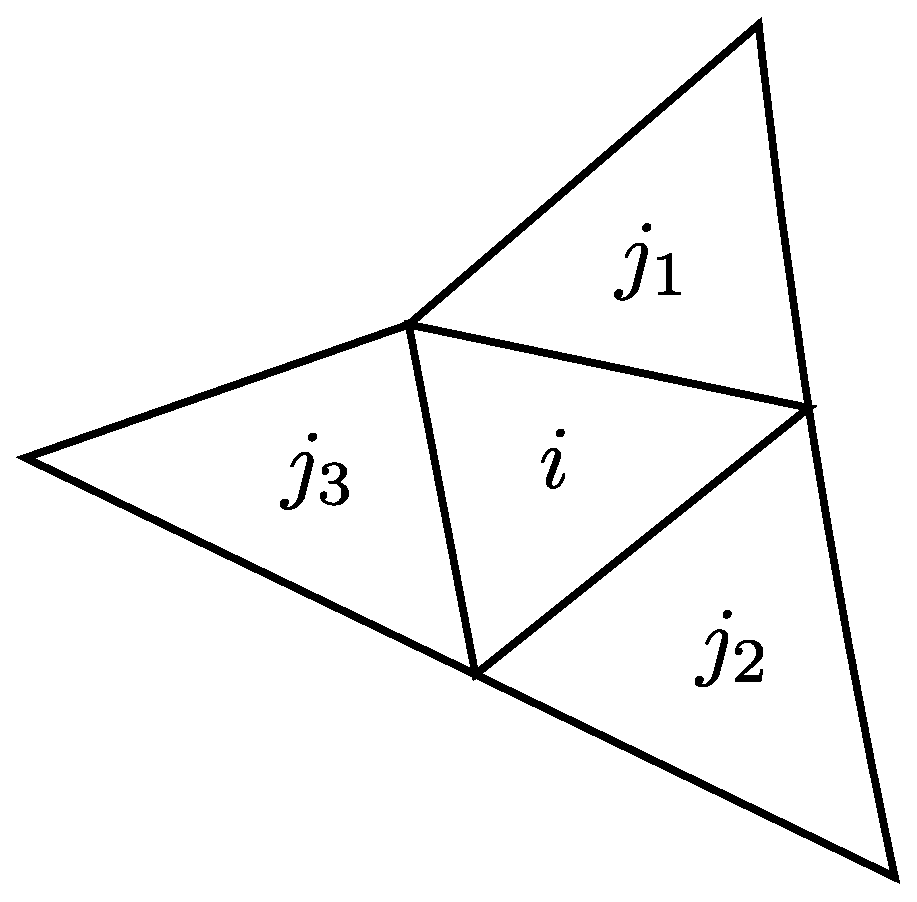
\includegraphics[width=0.43 \textwidth]{stencil3.eps}
		\label{fig:stencil:3}
	} 
	\subfigure[]{
		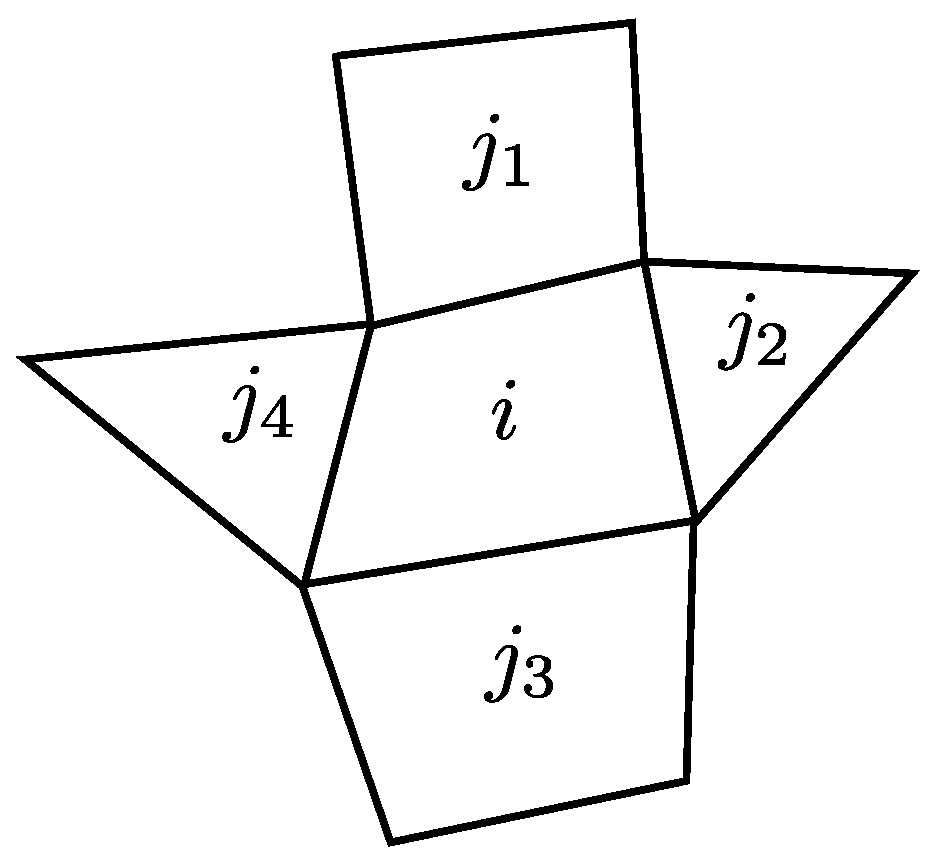
\includegraphics[width=0.47 \textwidth]{stencil4.eps}
		\label{fig:stencil:4}
	}
	\caption{Reconstruction stencil for cell i. (a) Stencil for a triangular cell. (b) Stencil for a quadrangular cell.}
	\label{fig:stencil}
\end{figure}

In the CLS reconstruction, the various orders of spatial derivatives of reconstruction polynomial $u(x,y)$ are required to be conserved on $S_i$ ($S_i=\{\Omega_1, \Omega_2, \cdots, \Omega_N\}$, $N$ denotes the total number of control volumes neighboring the cell $i$). Namely, for all $\Omega_j \in S_i$,
\begin{equation}\label{eq:spdConserved:1}
	\frac{1}{\|\Omega_j\|}\int_{\Omega_j}\frac{\partial^{m+n}u^i(x,y)}{\partial x^my^n}dxdy=\frac{1}{\|\Omega_j\|}\int_{\Omega_j}\frac{\partial^{m+n}u^j(x,y)}{\partial x^my^n}dxdy, \quad 0\leq m+n \leq M,
\end{equation}
where $M \leq k$. Substituting Eq.~\eqref{eq:RCP} into Eq.~\eqref{eq:spdConserved:1}, we obtain the following linear equations
\begin{equation}\label{eq:spdConserved:2}
	\begin{gathered}
		\sum_{l=1}^{DOF(k)}u^i_l\left(\frac{1}{\|\Omega_j\|}\int_{\Omega_j}\frac{\partial^{m+n}\phi_{l,i}(x,y)}{\partial x^my^n}dxdy\right)
		=\delta^0_{m+n}\left(\overline{u}^j-\overline{u}^i\right)\\
		+\sum_{l=1}^{DOF(k)}u^j_l\left(\frac{1}{\|\Omega_j\|}\int_{\Omega_j}\frac{\partial^{m+n}\phi_{l,j}(x,y)}{\partial x^my^n}dxdy\right).
	\end{gathered}
\end{equation}
Let
\begin{equation}\label{eq:u_i}
	\bm{u}^i=\left(u^i_1, u^i_2, \cdots ,u^i_{DOF(k)}\right)^T,
\end{equation}
Eq.~\eqref{eq:spdConserved:2} can be rewritten as
\begin{equation}\label{eq:spdConserved:3}
	\bm{A}^i_j\bm{u}^i-\bm{B}^i_j\bm{u}^j=\bm{b}^i_j,
\end{equation}
where
\begin{equation}\label{eq:A:B:b}
	\begin{gathered}
	\bm{A}^i_j=\left[\frac{1}{\|\Omega_j\|}\int_{\Omega_j}\frac{\partial^{m+n}\phi_{l,i}(x,y)}
		{\partial x^my^n}dxdy\right]_{(DOF(M)+1) \times DOF(k)},\\
	\bm{B}^i_j=\left[\frac{1}{\|\Omega_j\|}\int_{\Omega_j}\frac{\partial^{m+n}\phi_{l,j}(x,y)}
		{\partial x^my^n}dxdy\right]_{(DOF(M)+1) \times DOF(k)},\\
	\bm{b}^i_j=\left[\delta^0_{m+n}\left(\overline{u}_j-\overline{u}_i\right)\right]_{(DOF(M)+1) \times 1}.
	\end{gathered}
\end{equation}
\section{The construction of linear system}
In this section, the structure of the linear system is introduced.
\begin{itemize}
	\item The structure of matrix $\bm{A}$\\
		According to Eq.~\eqref{eq:A:B:b}, the matrix $A$ can be constructed as 
		\begin{equation}\label{eq:A}
			\bm{A}=\left[\bm{A}^1; \bm{A}^2; \cdots; \bm{A}^N\right],
		\end{equation}
		where $N$ represents the total number of the control volumes, and the superscript $i$ ($i=1,2, \cdots, N$) is related to the 
		certain control volume in the computational domain. $\bm{A}^i$ can be expressed as
		\begin{equation}\label{eq:Ai}
			\bm{A}^i=\left[\bm{A}^i_1; \bm{A}^i_2; \cdots; \bm{A}^i_{nNeighbor}\right],
		\end{equation}
		where the subscript $j$ ($j=1,2, \cdots, nNeighbor$) denotes the neighboring control volume. The structure of block matrix $\bm{A}^i_j$ can be exhibited as Figure \ref{fig:BlockAij}.

	\item The structure of matrix $\bm{B}$\\
		According to Eq.~\eqref{eq:A:B:b}, the matrix $B$ can be constructed as 
		\begin{equation}\label{eq:B}
		\bm{B}=\left[\bm{B}^1; \bm{B}^2; \cdots; \bm{B}^N\right],
		\end{equation}
		where $\bm{B}^i$ can be expressed as
		\begin{equation}\label{eq:Bi}
		\bm{B}^i=\left[\bm{B}^i_1; \bm{B}^i_2; \cdots; \bm{B}^i_{nNeighbor}\right].
		\end{equation}
		The structure of block matrix $\bm{B}^i_j$ can be exhibited as Figure \ref{fig:BlockBij}.

	\item The structure of vectors $\bm{b}$ and $\bm{u}$\\
		The vector $\bm{b}$ can be written as
		\begin{equation}\label{eq:b}
			\bm{b}=\{\bm{b}^1, \bm{b}^2, \cdots, \bm{b}^N\}^T,
		\end{equation}
		and the vector $\bm{u}$ reads as
		\begin{equation}\label{eq:u}
			\bm{u} = \{\bm{u}^1, \bm{u}^2, \cdots, \bm{u}^N\}^T.
		\end{equation}
		The structures of vectors $\bm{b}$ and $\bm{u}$ can be referred to Figure \ref{fig:BlockAij} and \ref{fig:BlockBij}.
\end{itemize}

\begin{figure}[!htp]
	\centering
	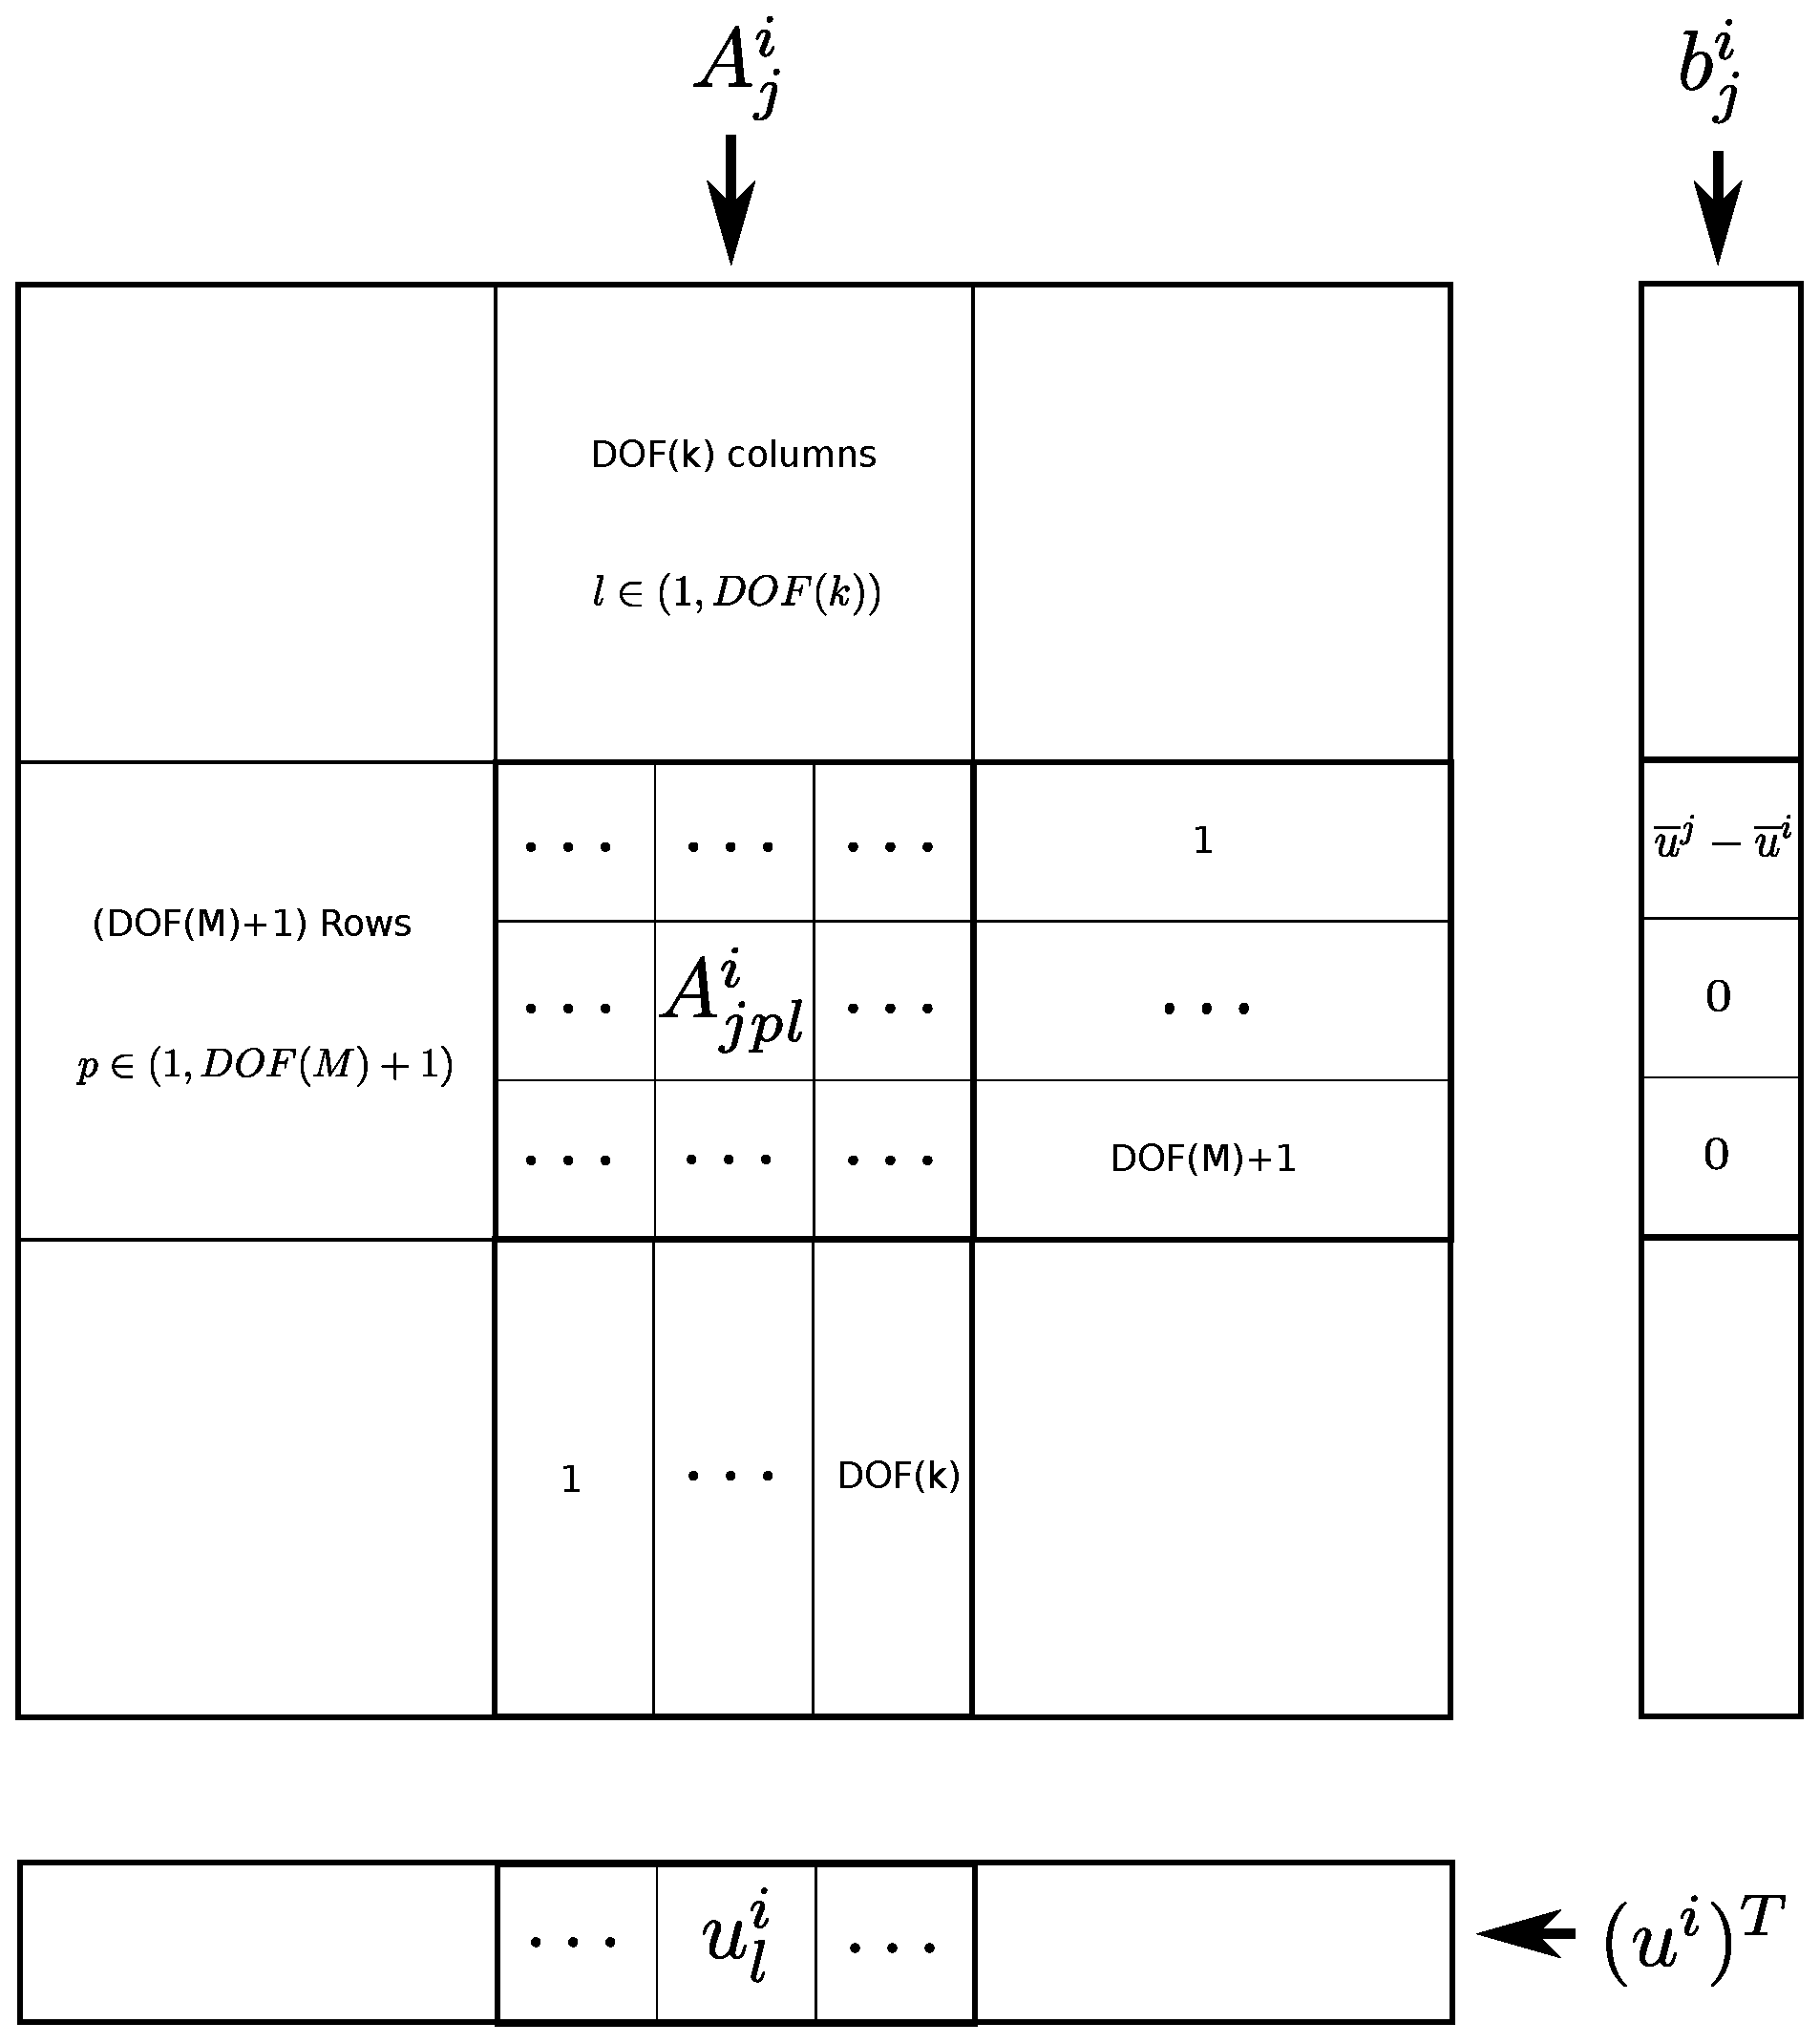
\includegraphics[width=0.8\textwidth]{Aij.eps}
	\caption{The structure of block matrix $A^i_j$.}
	\label{fig:BlockAij}
\end{figure}

\begin{figure}[!htp]
	\centering
	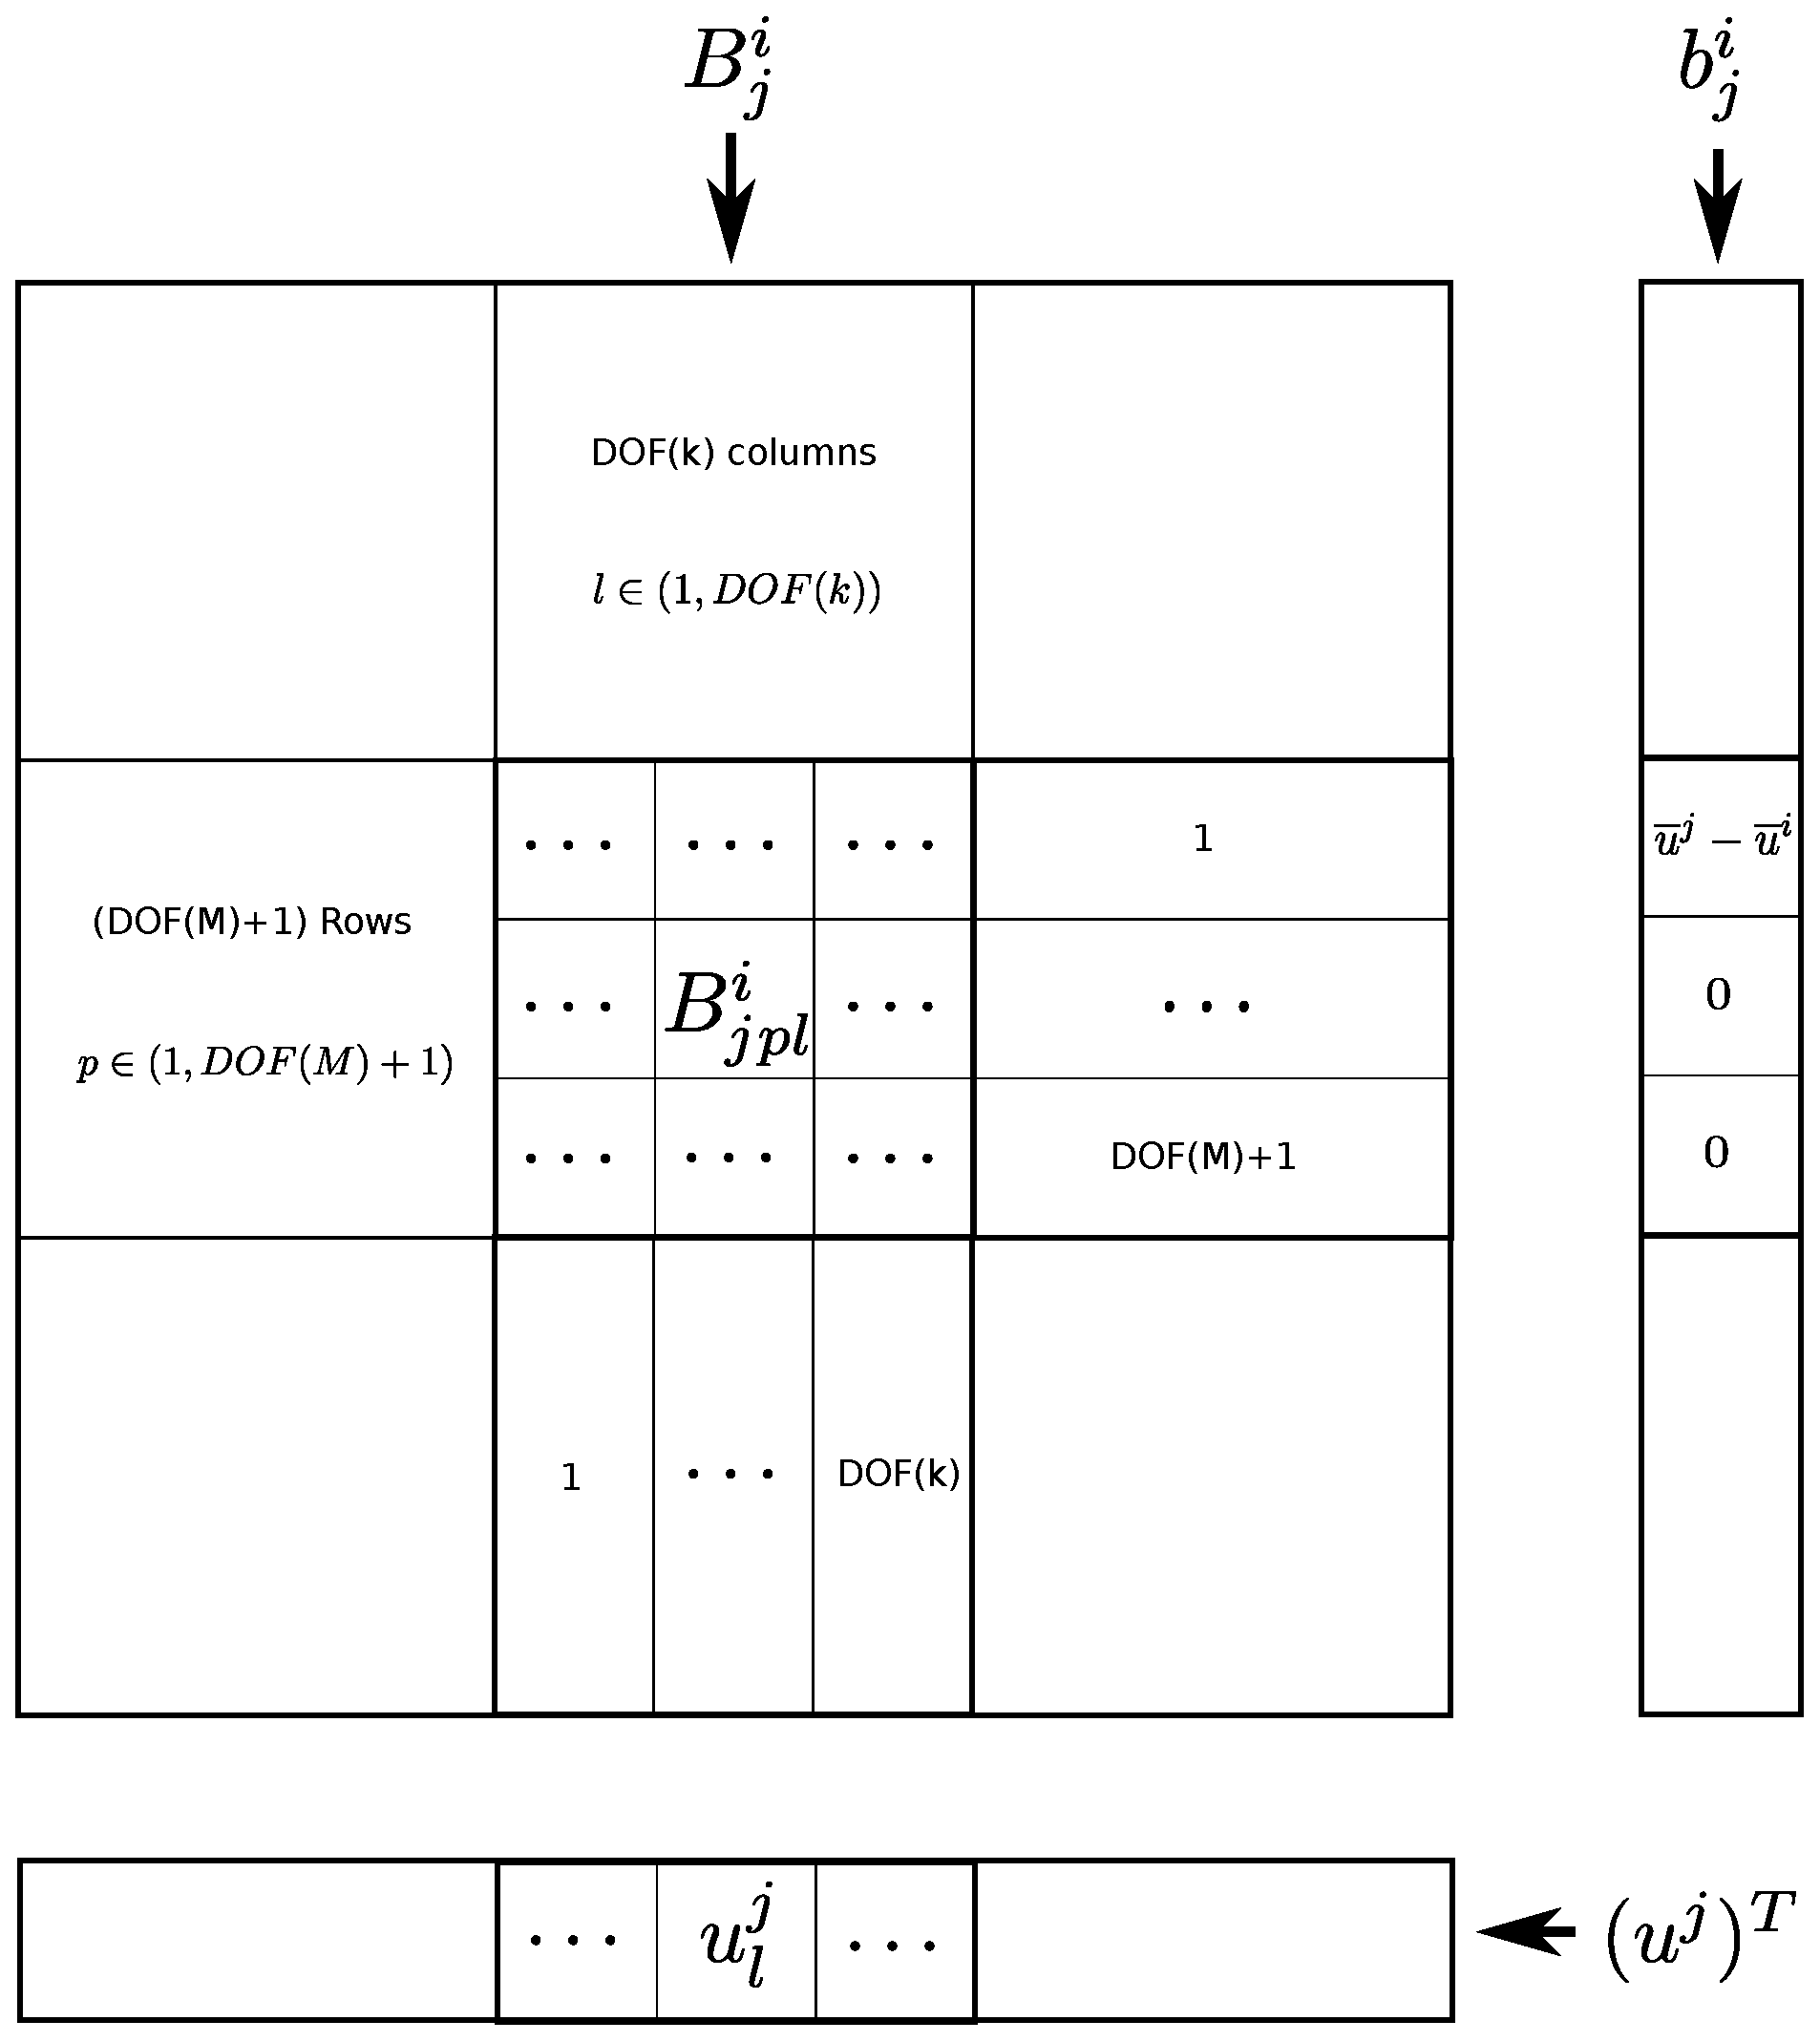
\includegraphics[width=0.8\textwidth]{Bij.eps}
	\caption{The structure of block matrix $B^i_j$.}
	\label{fig:BlockBij}
\end{figure}

\section{WBAP high order limiter}
	To suppress the non-physical oscillations near the discontinuities, the WBAP limiter is applied.
	\begin{equation}\label{eq:wbap}
		W=W^{L2}(1, \theta_1, \cdots, \theta_J)=\frac{n_p+\sum_{k=1}^{J}{1/\theta_{k}^{p-1}}}{n_p+\sum_{k=1}^{J}{1/\theta_{k}^{p}}},
	\end{equation}
	where $p = 4$ and $n_p = 10$.
	The secondary reconstruction coefficients are
	\begin{equation}\label{eq:uji}
		\begin{gathered}
			u_{j \cdot i}^l=\frac{h_i^2}{h_j^2}u_j^l, \quad l=3,4,5,\\
			u_{j \cdot i}^2=\frac{h_i}{h_j}u_j^2+\frac{h_i}{h_j}\frac{x_i-x_j}{h_j}u_j^4
				+\frac{2h_i}{h_j}\frac{y_i-y_j}{h_j}u_j^5,\\
			u_{j \cdot i}^1=\frac{h_i}{h_j}u_j^1+\frac{2h_i}{h_j}\frac{x_i-x_j}{h_j}u_j^3
			+\frac{h_i}{h_j}\frac{y_i-y_j}{h_j}u_j^4,
		\end{gathered}
	\end{equation}
	and $\theta_k = \frac{u_{k \cdot i}^l}{u_i^l}$
\section {3 order clsfv reconstruction}
	For 3 order clsfv reconstruction,
	\begin{equation}\label{3orderParameters}
		k=2, \quad, DOF(k)=5, \quad M=k-1=1, DOF(M)=2.
	\end{equation}
	Let
	\begin{equation}\label{avgj}
		<\Delta x^m_i\Delta y^n_i>=\frac{1}{\|\Omega_j\|}\int_{\Omega_j}\Delta x^m_i\Delta y^n_id\Omega,
	\end{equation}
	and the $\bm{A}^i_{jpl}$ and $\bm{B}^i_{jpl}$ can be obtained from tables \ref{tab:Aijpl} and \ref{tab:Bijpl}.
	\begin{table}[!htp]
		\centering
		\caption{\label{tab:Aijpl} Summary of $\bm{A}^i_{jpl}$.}
		\begin{threeparttable}
			\begin{tabular}{p{100pt} p{100pt}<{\centering} p{80pt}<{\centering} p{80pt}<{\centering} p{80pt}<{\centering} p{80pt}<{\centering}}
				\hline
				\hline
				 & $p=0$ & $p=1$ & $p=2$ \\
				\hline
				 & $m=0, n=0$ & $m=1, n=0$ & $m=0, n=1$ \\
				\hline
				& $\bm{A}^i_{j0l}$ & $\bm{A}^i_{j1l}$ & $\bm{A}^i_{j2l}$ \\
				\hline
				$l=1$ & $<\Delta x_i>-\overline{\Delta x_i}$ & $\frac{1}{h_i}$ & $0$ \\
				
				$l=2$ & $<\Delta y_i>-\overline{\Delta y_i}$ & $0$ & $\frac{1}{h_i}$\\
				
				$l=3$ & $<\Delta x^2_i>-\overline{\Delta x^2_i}$ & $\frac{2<\Delta x_i>}{h_i}$ & $0$\\
				
				$l=4$ & $<\Delta x_i\Delta y_i>-\overline{\Delta x_i\Delta y_i}$ & $\frac{<\Delta y_i>}{h_i}$ & $\frac{<\Delta x_i>}{h_i}$\\
				
				$l=5$ & $<\Delta y^2_i>-\overline{\Delta y^2_i}$ & $0$ & $\frac{2<\Delta y_i>}{h_i}$\\
				\lasthline
			\end{tabular}
		\end{threeparttable}
	\end{table}
	\begin{table}[!htp]
		\centering
		\caption{\label{tab:Bijpl} Summary of $\bm{B}^i_{jpl}$.}
		\begin{threeparttable}
			\begin{tabular}{p{100pt} p{100pt}<{\centering} p{80pt}<{\centering} p{80pt}<{\centering} p{80pt}<{\centering} p{80pt}<{\centering}}
				\hline
				\hline
				& $p=0$ & $p=1$ & $p=2$ \\
				\hline
				& $m=0, n=0$ & $m=1, n=0$ & $m=0, n=1$ \\
				\hline
				& $\bm{B}^i_{j0l}$ & $\bm{B}^i_{j1l}$ & $\bm{B}^i_{j2l}$ \\
				\hline
				$l=1$ & $0$ & $\frac{1}{h_j}$ & $0$ \\
				
				$l=2$ & $0$ & $0$ & $\frac{1}{h_j}$\\
				
				$l=3$ & $0$ & $\frac{2\overline{\Delta x_j}}{h_j}$ & $0$\\
				
				$l=4$ & $0$ & $\frac{\overline{\Delta y_j}}{h_j}$ & $\frac{\overline{\Delta x_j}}{h_j}$\\
				
				$l=5$ & $0$ & $0$ & $\frac{2\overline{\Delta y_j}}{h_j}$\\
				\lasthline
			\end{tabular}
		\end{threeparttable}
	\end{table}
\section {Some notes for validation of a 4x4 Cartesian grid}
To validate the construction of sparse matrix $\bm{A}$ and $\bm{B}$, we take a $4 \times 4$ Cartesian grid as an example.
The computational domain is $(0, 1) \times (0,1)$, and the grid is shown as Figure \ref{fig:grid4x4}.  
\begin{figure}[!htp]
	\centering
	\subfigure[]{
		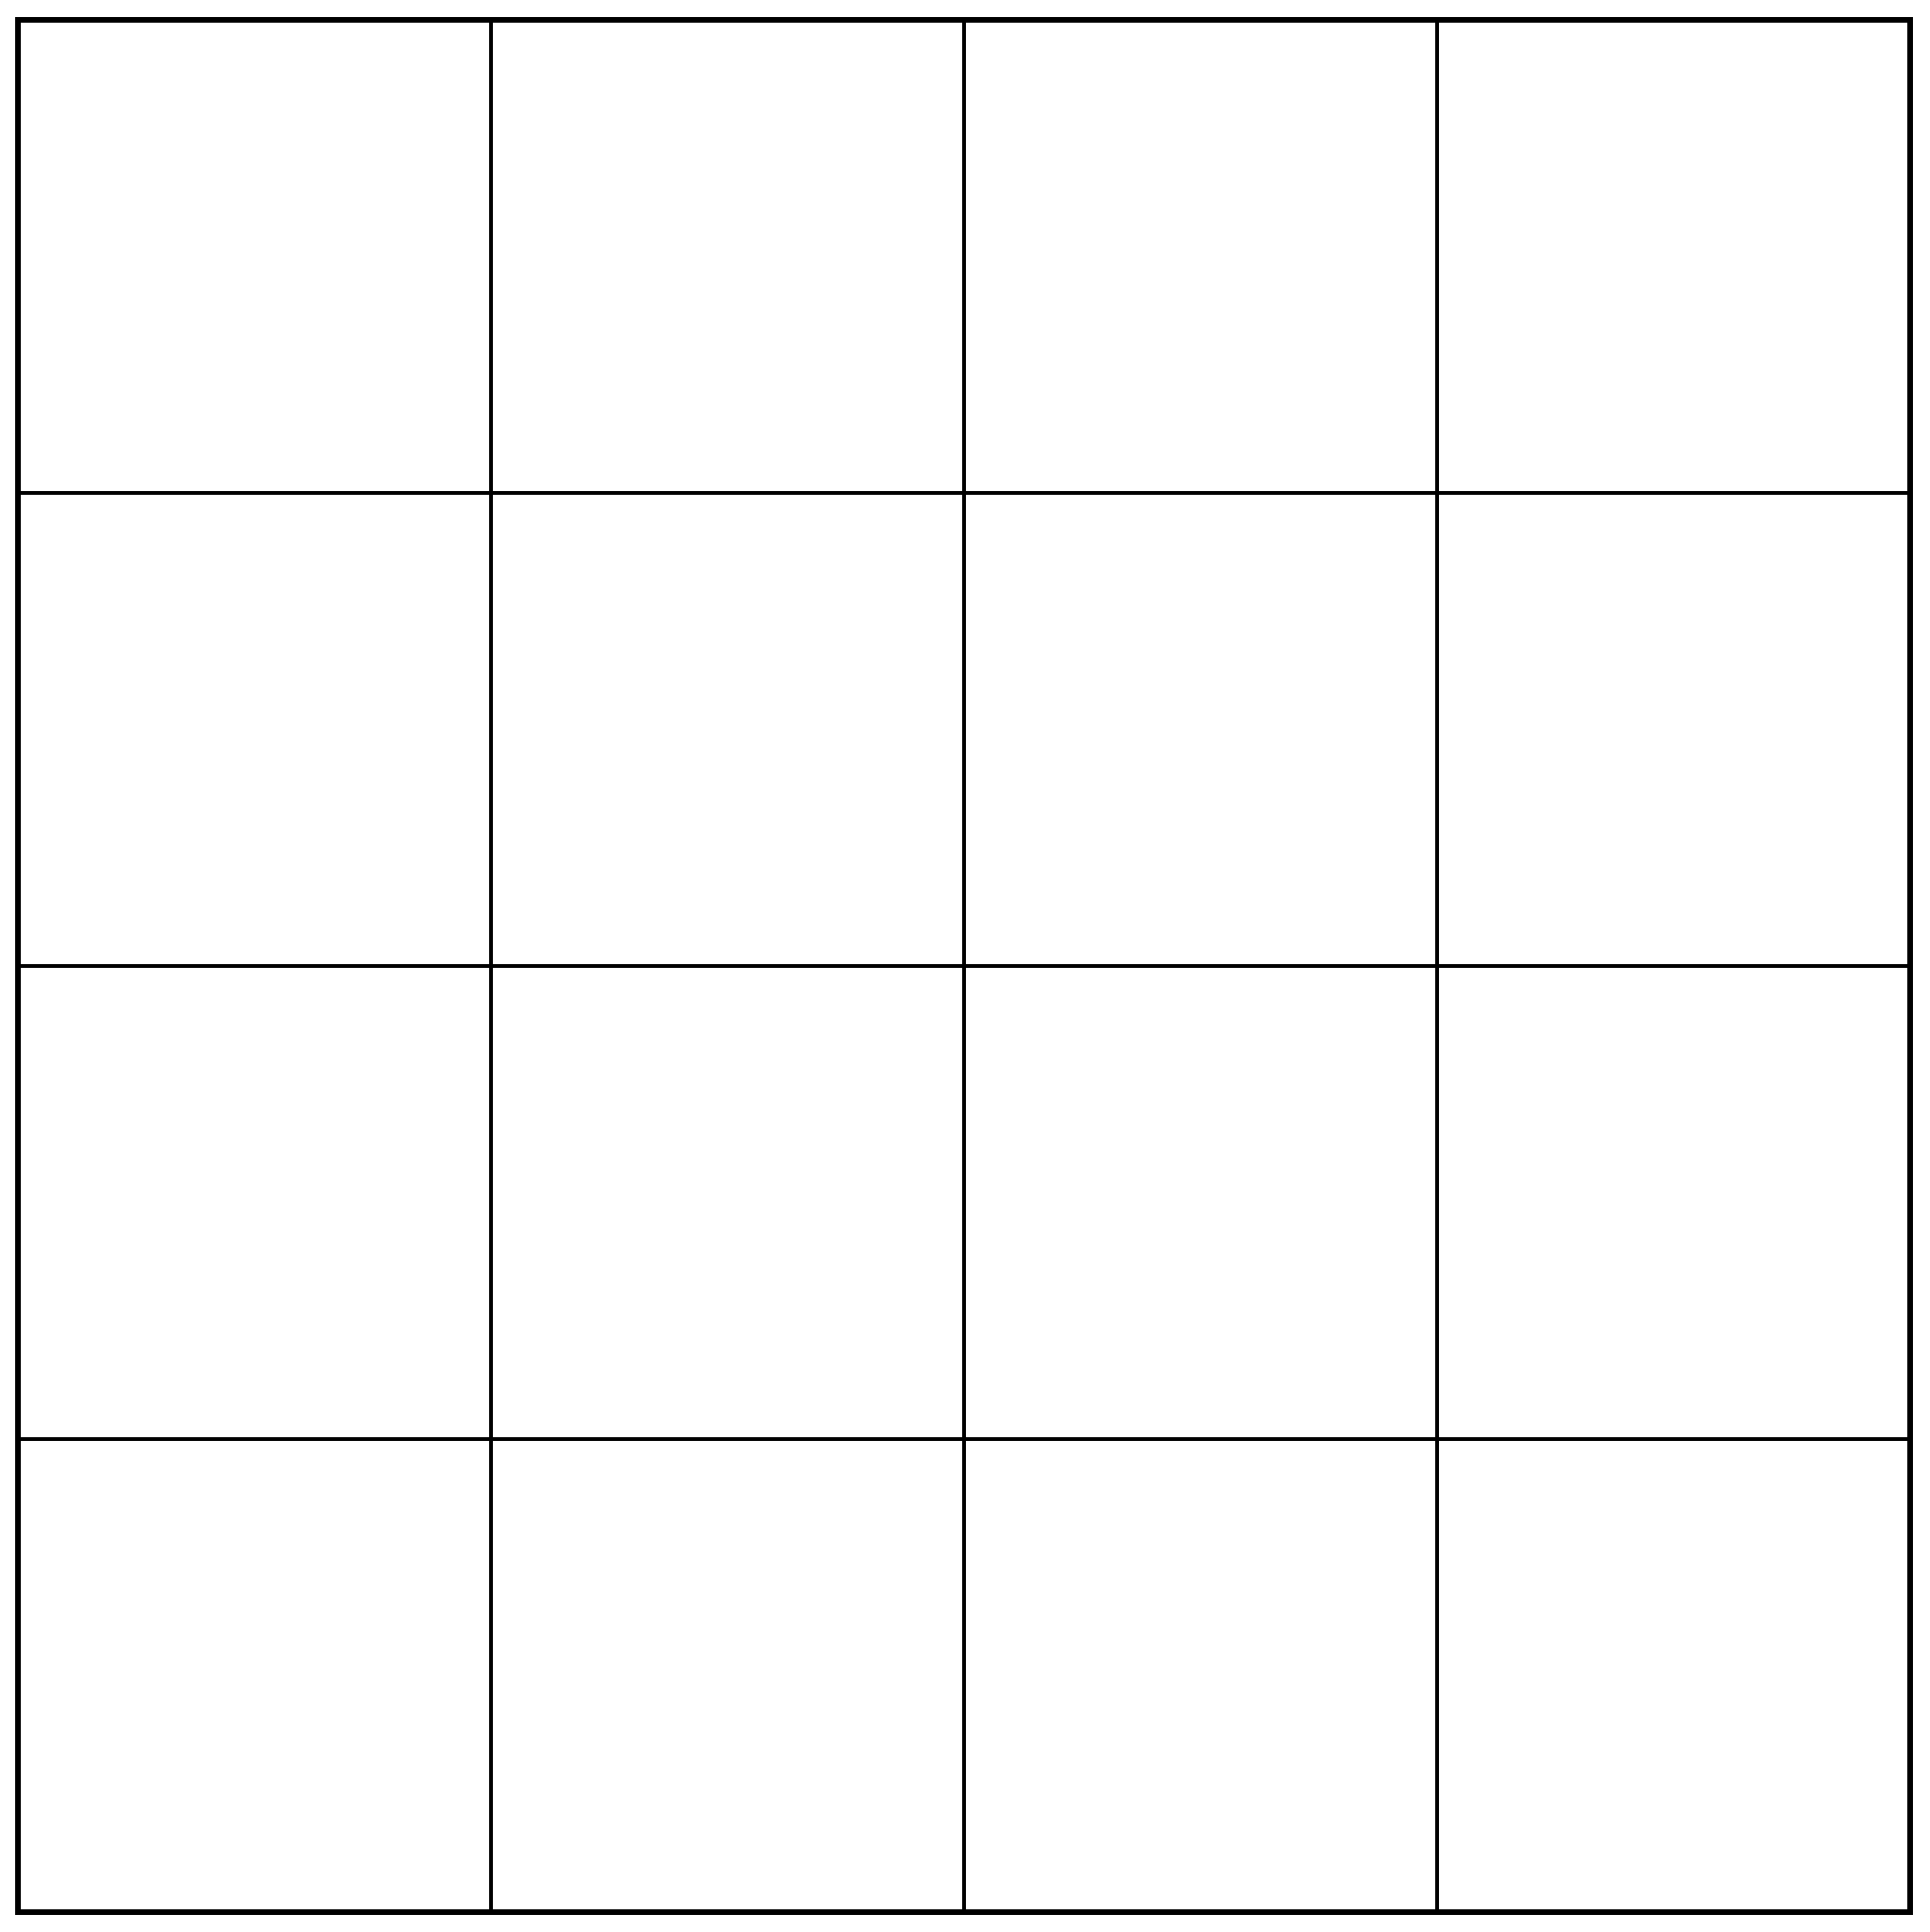
\includegraphics[width=0.45 \textwidth]{grid4x4.eps}
		\label{fig:grid4x4_1}
	} 
	\subfigure[]{
		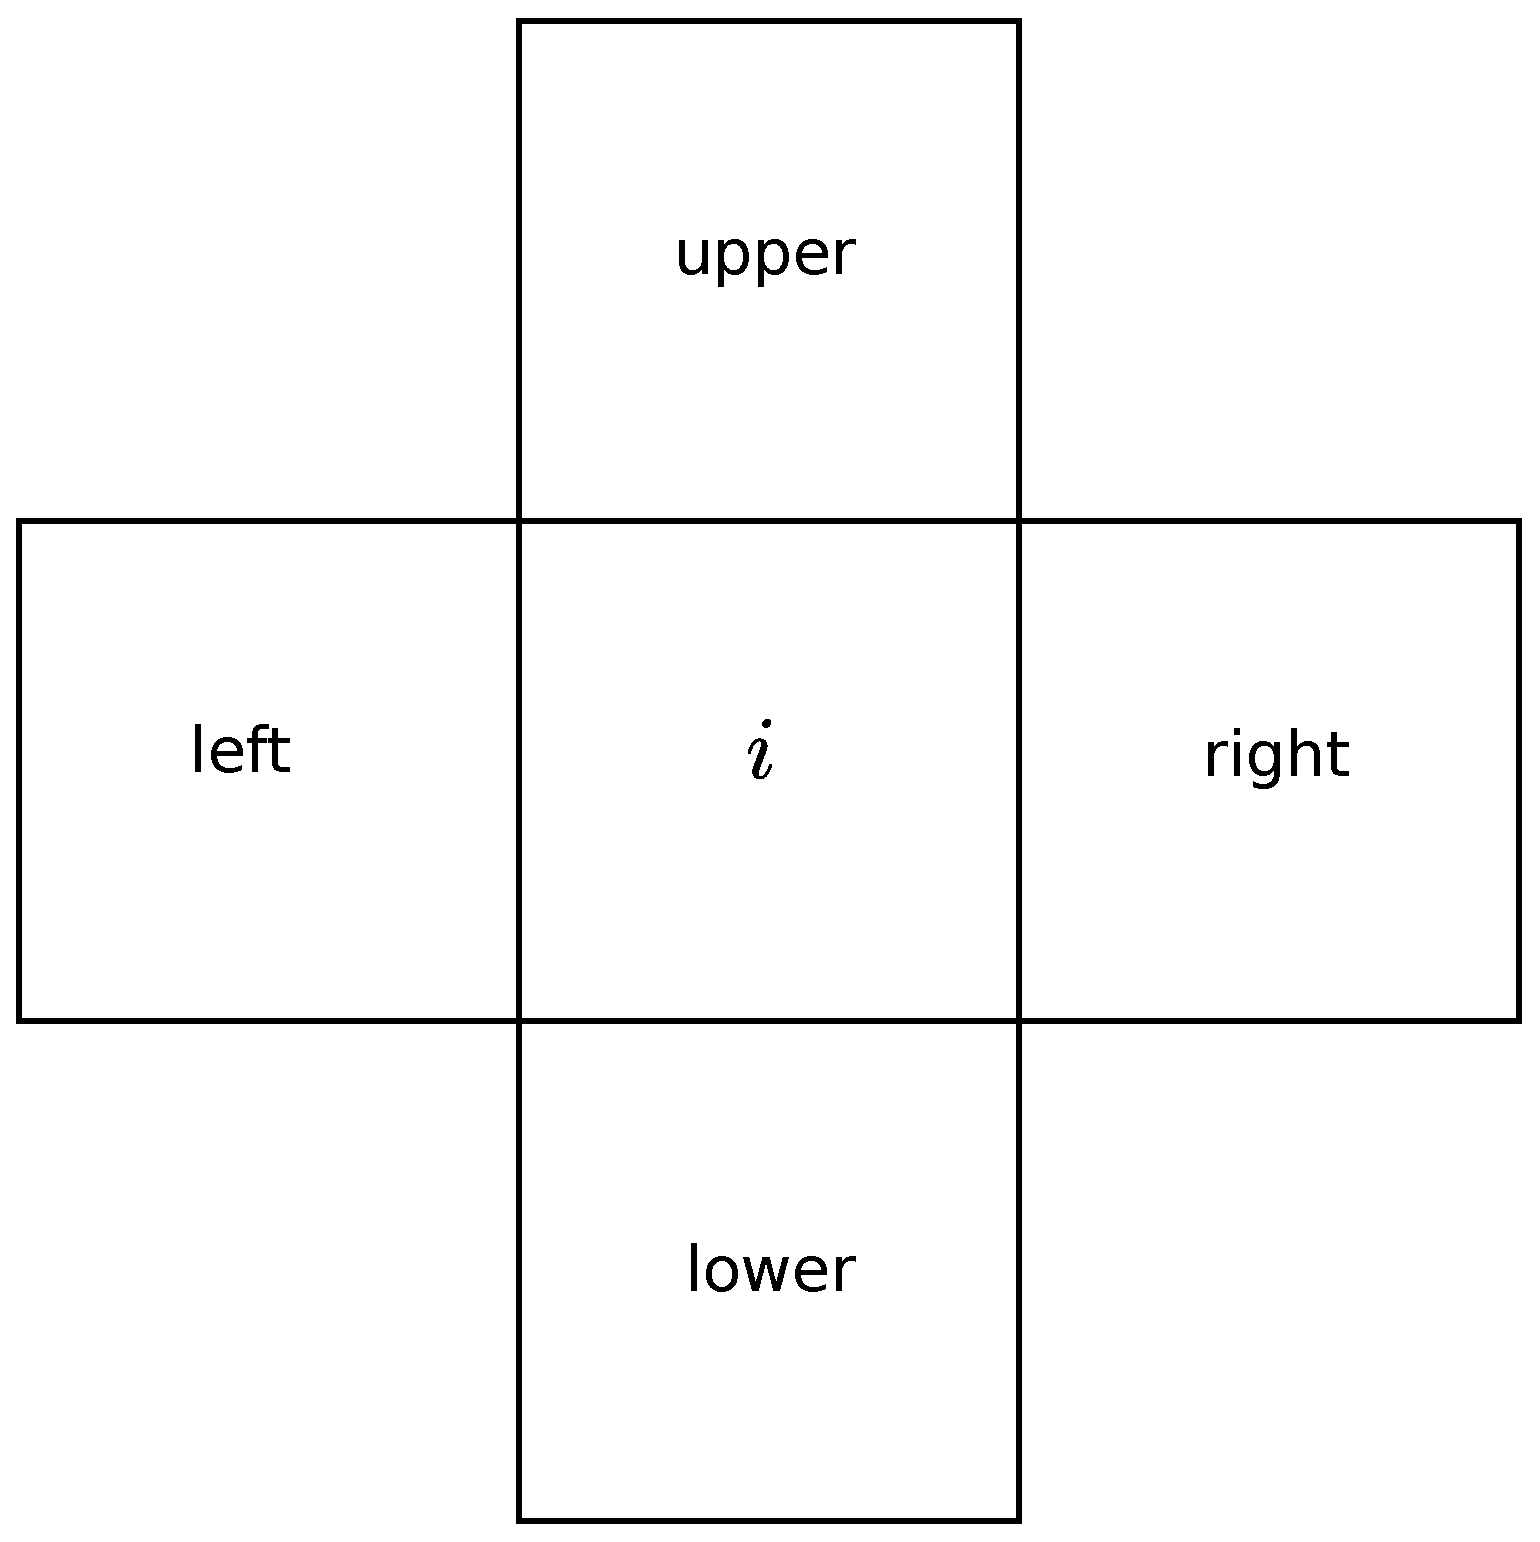
\includegraphics[width=0.45 \textwidth]{neighbor.eps}
		\label{fig:neighbor}
	}
	\caption{The $4 \times 4$ Cartesian grid. (a) $4 \times 4$ Cartesian grid. (b) Neighboring cells of control volume $i$.}
	\label{fig:grid4x4}
\end{figure}
Let
\begin{equation}\label{exLinearSys}
	\bm{A}=\bm{A}_{nRow,nCol}, \quad \bm{B}=\bm{B}_{nRow,nCol}, \quad \bm{b}=\bm{b}_{nRow}, \quad \bm{u}=\bm{u}_{nCol},
\end{equation}
where $nRow=80$ and $nCol=44$. The average values of $\overline{\Delta x^m\Delta y^n}$ are
\begin{equation}\label{eq:avgi}
	\overline{\Delta x_i} = 0, \quad \overline{\Delta y_i}=0, \quad \overline{\Delta x^2_i} = 0.0833333, 
	\quad \overline{\Delta x_i\Delta y_i} = 0, \quad \overline{\Delta y^2_i} = 0.0833333, 
\end{equation}
and $h_i=0.25$. The average values $<\Delta x^m\Delta y^n>$ can be found in table \ref{tab:avgj}.
	\begin{table}[!htp]
		\centering
		\caption{\label{tab:avgj} Summary of $<\Delta x^m\Delta y^n>$.}
		\begin{threeparttable}
			\begin{tabular}{p{60pt} p{100pt}<{\centering} p{80pt}<{\centering} p{80pt}<{\centering} p{80pt}<{\centering} p{80pt}<{\centering}}
				\hline
				\hline
				& left & upper & right & lower \\
				\hline
				$<\Delta x_i>$ & $-1$ & $0$ & $1$ & $0$ \\
				
				$<\Delta y_i>$ & $0$ & $1$ & $0$ & $-1$\\
				
				$<\Delta x^2_i>$ & $1.0833333$ & $0.0833333$ & $1.0833333$ & $0.0833333$\\
				
				$<\Delta x_i\Delta y_i>$ & $0$ & $0$ & $0$ & $0$\\
				
				$<\Delta y^2_i>$ & $0.0833333$ & $1.0833333$ & $0.0833333$ & $1.0833333$\\
				\lasthline
			\end{tabular}
		\end{threeparttable}
	\end{table}
\end{document}
